\documentclass[10pt]{beamer}

\usetheme[progressbar=frametitle]{metropolis}

\usepackage{booktabs}
\usepackage[scale=2]{ccicons}

\usepackage{graphicx}
\usepackage[outdir=./img/]{epstopdf}
\epstopdfsetup{update}


\usepackage{pgfplots}
\usepgfplotslibrary{dateplot}
\usepackage{movie15}


\usepackage{xspace}
\newcommand{\themename}{\textbf{\textsc{metropolis}}\xspace}

\usepackage{hyperref}

\title{Douglass-Peucker Algorithm}
\subtitle{A simplification of polyline}
\date{\today}
\author{Banyas Miron}
\institute{Kyiv Algorithms Club}
\titlegraphic{\hfill
\includegraphics[height=3cm]{img/logo}}


\begin{document}

\maketitle

\begin{frame}{Table of contents}
  \setbeamertemplate{section in toc}[sections numbered]
  \tableofcontents[hideallsubsections]
\end{frame}

\section{Introduction}

\begin{frame}{Application}
	\begin{itemize}
		\item \textbf{Cartography:} map generalization.
		\item \textbf{Vector graphics.}
		\item \textbf{Robotics:} denoising of range data acquired by a rotating range scanner. 
	\end{itemize}
\end{frame}

\begin{frame}{Map Generalization}
	\begin{figure}[h]
			\center{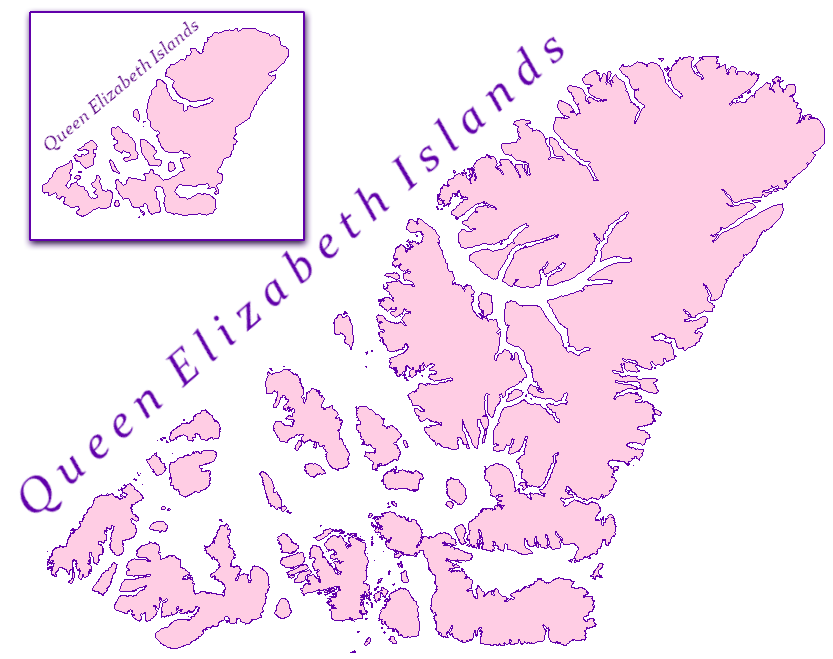
\includegraphics[width=0.8\linewidth]{img/app01.png}}
		\end{figure}
\end{frame}

\begin{frame}{Map Generalization}
	\begin{figure}[h]
			\center{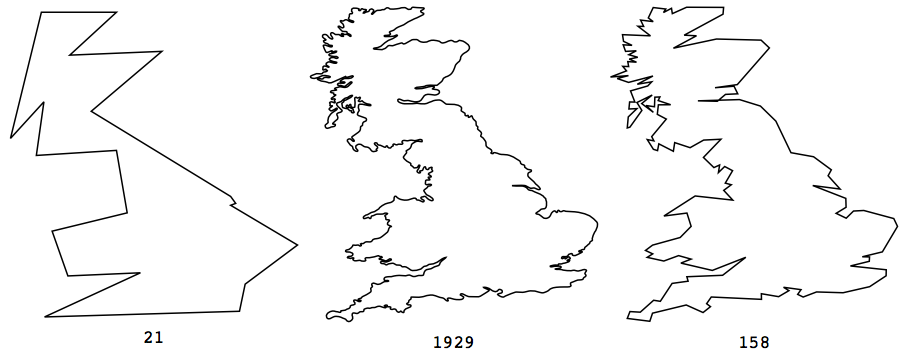
\includegraphics[width=0.8\linewidth]{img/app02.png}}
		\end{figure}
\end{frame}

\begin{frame}{Map Generalization}
	\begin{figure}[h]
			\center{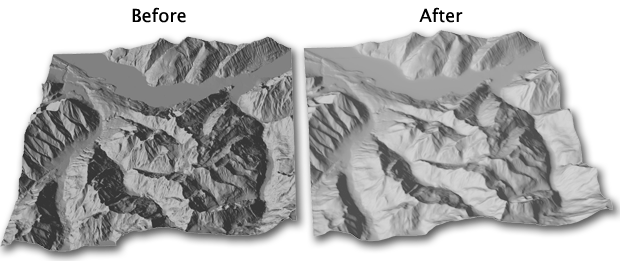
\includegraphics[width=1.0\linewidth]{img/app03.jpg}}
		\end{figure}
\end{frame}



\begin{frame}{Resources}
	\begin{itemize}
		\item \textit{C++ polyline simplification library and demo application} -- \url{http://psimpl.sourceforge.net/} 
		\item \textit{JavaScript polyline simplification library} --  \url{http://mourner.github.io/simplify-js/}
		\item \textit{Java implementation of DPA} -- \url{https://github.com/hgoebl/simplify-java}	
		\item \textit{Matlab implementation of DPA} -- \url{https://www.mathworks.com/matlabcentral/fileexchange/21132-line-simplification/content/dpsimplify.m}	
	\end{itemize}
\end{frame}
\begin{frame}{References}
	\begin{itemize}
		\item Urs Ramer 
		 	  "An iterative procedure for the polygonal approximation of plane curves", 
   			  \textit{Computer Graphics and Image Processing}, 1(3), 244–256 (1972)
		\item David Douglas \& Thomas Peucker, 
			  "Algorithms for the reduction of the number of points required to represent a digitized line or its caricature", 
			  \textit{The Canadian Cartographer} 10(2), 112–122 (1973)
		\item J.L.G. Pallero
			  Robust line simplification on the plane
			  \textit{Computers \& Geosciences} 61 (2013) 
	\end{itemize}
\end{frame}

\section{Basic Idea}

\begin{frame}{Problem}
Given a simple polygonal chain $P$  (a polyline) defined by a sequence of points $p_{1},p_{2},...,p_{n}$ in the plane. 

\begin{alertblock}{Goal}
Produce a simplified polyline  $Q=\{p_{i_{1}},p_{i_{2}},...,p_{i_{k}}\}$
that for each point $p_{l}\in P$ the distance $\rho$ between $p_{l}$
and the segment $\overline{p_{i_{j}}p_{i_{j+1}}}$ ($i_{j} < l < i_{j+1}$) 
is less or equal a given tolerance $\varepsilon$.
\end{alertblock}

\begin{alertblock}{Alternative Goal}
Produce a simplified polyline  $Q=\{p_{i_{1}},p_{i_{2}},...,p_{i_{k}}\}$
that for each point $p_{l}\in P$ the distance $\rho$ between $p_{l}$
and the segment $\overline{p_{i_{j}}p_{i_{j+1}}}$ ($i_{j} < l < i_{j+1}$)   
is  minimal for a given number $k$.
\end{alertblock}

\end{frame}

\begin{frame}{Problem Solving}
	\begin{itemize}
		\item %The first and the last point in the original polyline are considered fixed.
			  %These two fixed points linked form a straight line that will be called a \alert{base segment}.		
			  The first and the last point ($p_{s}$ and $p_{e}$)  in the original polyline 
			  linked form a straight line $\overline{p_sp_e}$ that will be called a \alert{base segment}.		
		\item %The distances between each remaining point in the original line
			  %and the base segment defined in the previous step are
			  %computed. The points considered from the original line in this
			  %step are those between the points that form the base segment.
			  The point $p_k$ ($s <  k < e$) with a maximal distance $\rho_{max}$ 
			  to the base segment defined in the previous step is found. 
		\item %The algorithm goes back to the first step, and considers now all
			  %the previously added vertices to the output line as fixed (the
			  %first and the last ones from the original line included). All of
			  %them, linked in pairs (in order from beginning to end) make up
		      %the new base segments.	
		      If $\rho_{max} \geq \varepsilon$ the resulting polyline is computed 
		      as a union of algorithm results on $\overline{p_{s}p_k}$ 
		      and $\overline{p_kp_{e}}$   base segment.
		\item %When no more points belonging to the original polyline are
			  %farther away than the tolerance from the correspondent base
			  %segment, the algorithm concludes.      
			  Otherwise the algorithm returns the base segment $\overline{p_sp_e}$.
	\end{itemize}
\end{frame}

\begin{frame}{Step by Step}
	\begin{figure}[h]
			\center{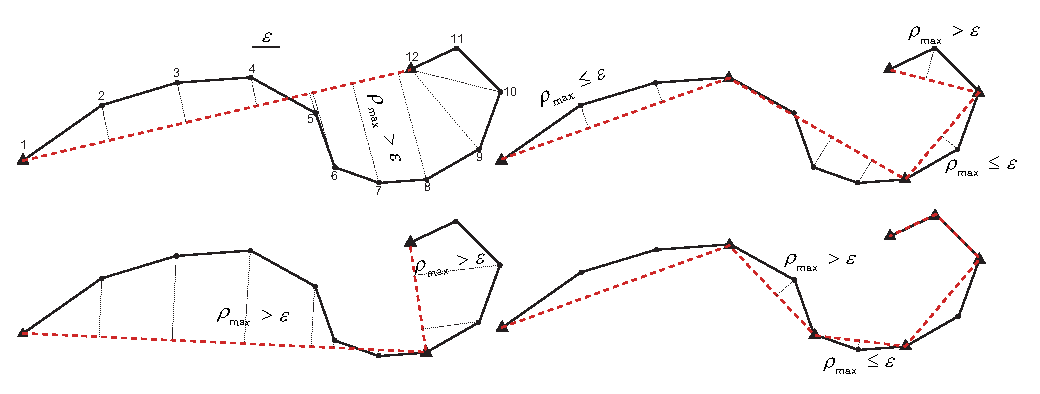
\includegraphics[width=1.\linewidth]{img/simple.eps}}
		\end{figure}
\end{frame}

\begin{frame}{Solving of the Alternative Problem}
	The solving of the alternative problem is similar to the initial technique.
	\begin{itemize}
		\item At each iteration the algorithm finds the base segment with a maximal distance
		and divides it, as in the original algorithm. The resulting base segments are kept
		for the subsequent iterations.
		\item It is useful to use a priority queue for storage of base segments.  
	\end{itemize}
	
\end{frame}

\section{Distance to a segment}

\begin{frame}{Vectors}

		\begin{figure}[h]
			\center{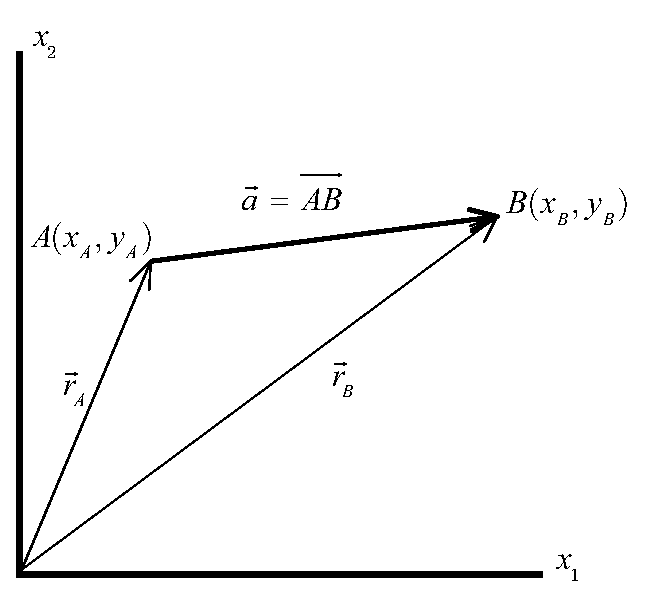
\includegraphics[width=0.5\linewidth]{img/vectors-1.eps}}
		\end{figure}
		
		\begin{align*}
				\overrightarrow{a} & = \overrightarrow{AB} = \overrightarrow{r_B} - \overrightarrow{r_A} \\
				 & = (x_B-x_A,y_B-y_A) = (x_a,y_a) 	
		\end{align*}


\end{frame}

\begin{frame}{Scalar Product}
		\begin{figure}[h]
			\center{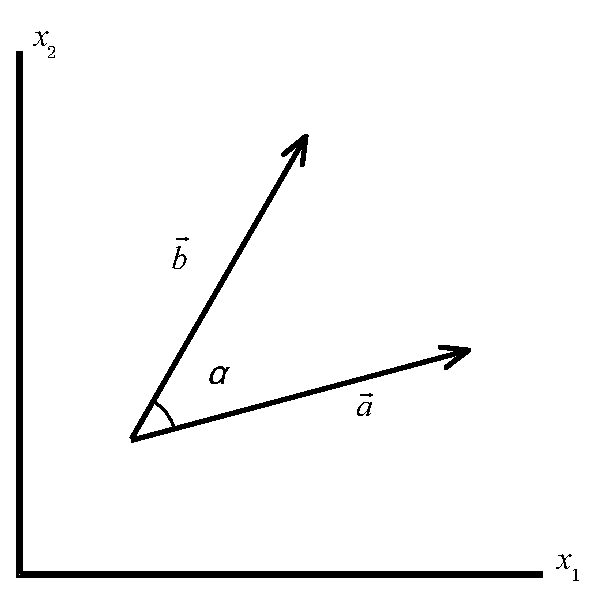
\includegraphics[width=0.5\linewidth]{img/vectors-2.eps}}
		\end{figure}
		\begin{align*}
				\overrightarrow{a} \cdot \overrightarrow{b} & = |\overrightarrow{a}||\overrightarrow{b}|\cdot\cos\alpha 
				= x_a x_b + y_a y_b 
		\end{align*}
		\begin{align*}
				|\overrightarrow{a}| = \sqrt{\overrightarrow{a} \cdot \overrightarrow{a}} = \sqrt{x_a^2 + y_a^2}
		\end{align*}
\end{frame}

\begin{frame}{Vector Product}
		\begin{figure}[h]
			\center{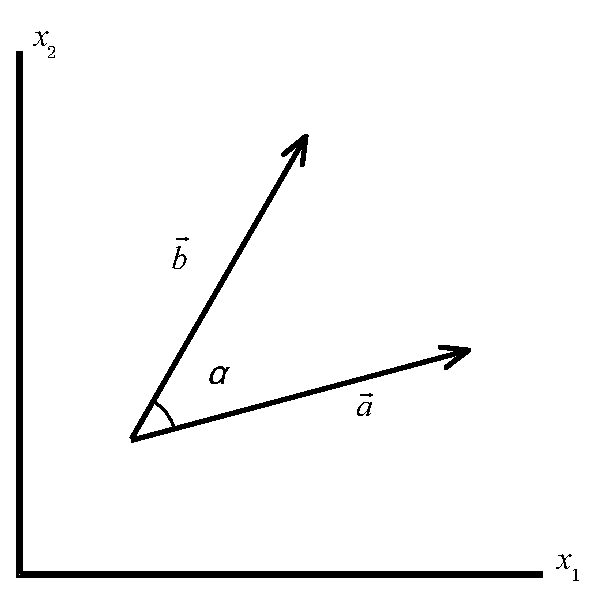
\includegraphics[width=0.5\linewidth]{img/vectors-2.eps}}
		\end{figure}
		\begin{align*}
				\overrightarrow{a} \times \overrightarrow{b} & = |\overrightarrow{a}||\overrightarrow{b}|\cdot\sin\alpha \\
				& = x_a y_b  - y_a x_b  
		\end{align*}
\end{frame}

\begin{frame}{Distance}
		\begin{figure}[h]
			\center{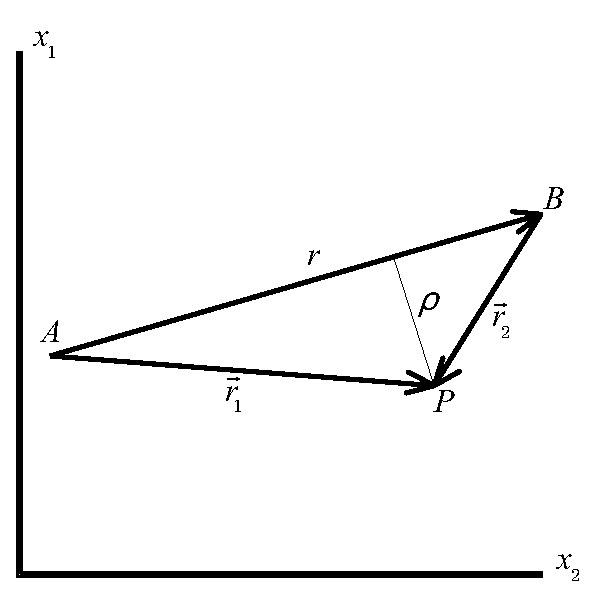
\includegraphics[width=0.5\linewidth]{img/vectors-3.eps}}
		\end{figure}
		\begin{align*}
				\rho  = |\overrightarrow{r_1}|\sin\alpha = |\overrightarrow{r_1}|\frac{|r\times r_1|}{|r|}
		\end{align*}
\end{frame}
\begin{frame}{Improving}
		\begin{figure}[h]
			\center{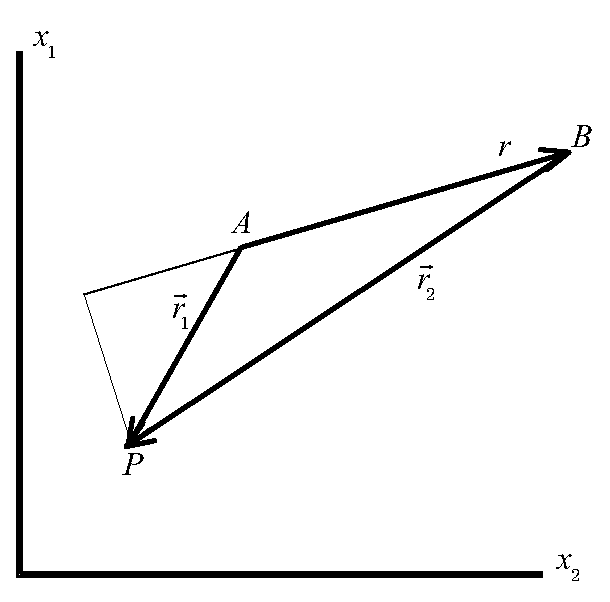
\includegraphics[width=0.5\linewidth]{img/vectors-4.eps}}
		\end{figure}
			\begin{itemize}
				\item{ \makebox[5cm]{if $r_2 >= \sqrt{r_1^2 + r^2}$} then $\rho=r_1$}
				\item{ \makebox[5cm]{if $r_1 >= \sqrt{r_2^2 + r^2}$} then $\rho=r_2$}
				\item{ \makebox[2.5cm]{} else $\rho = |\overrightarrow{r_1}|\frac{|r\times r_1|}{|r|}$}
			\end{itemize}
\end{frame}

\section{Algorithm features}

\begin{frame}{Complexity}
	The expected complexity of this algorithm can be described by the linear recurrence
	$$
		T(n) = 2 T(n/2)+O(n)
	$$
	Using the \textbf{Master Theorem} we can find that the complexity is
	$$
		T(n) \in \Theta(n \log(n))
	$$ 
	The \textbf{worst-case} complexity is $O(n^2)$	  
\end{frame}

\begin{frame}{Optimality}
	The Douglas-Peucker algorithm is not optimal with respect to the number of points.
	\begin{figure}[h]
		\begin{minipage}[h]{0.49\linewidth}
			\center{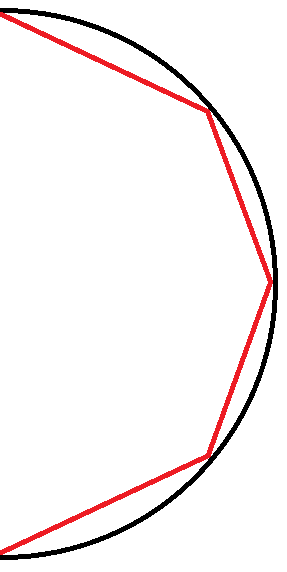
\includegraphics[width=0.5\linewidth]{img/non-optimal.png} \\ The answer of Douglas-Peucker Algorithm}
		\end{minipage}
		\hfill
		\begin{minipage}[h]{0.49\linewidth}
			\center{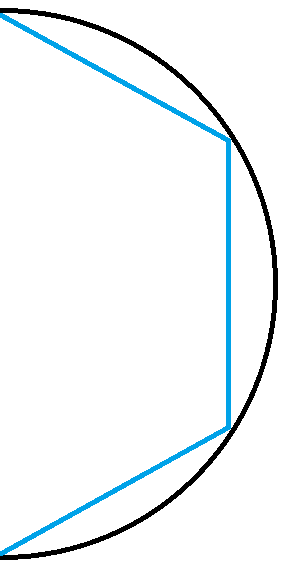
\includegraphics[width=0.5\linewidth]{img/optimal.png} \\ The optimal answer with respect to the number of points}
		\end{minipage}
	\end{figure}
\end{frame}
	
\begin{frame}{Robust}
	The Douglas-Peucker technique would have to be considered a non-robust algorithm
	since the resulting polyline may contain self-intersections.
	\begin{figure}[h]
			\center{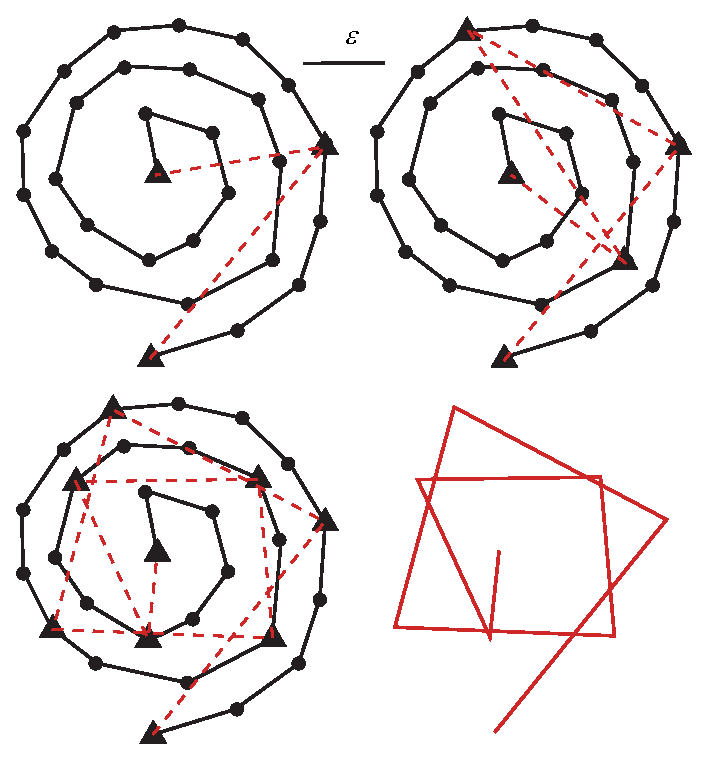
\includegraphics[width=0.5\linewidth]{img/simple_intersection.eps}}
	\end{figure}
\end{frame}

\section{Robust algorithm}

\begin{frame}{Non-Recursive Non-Robust Variant}
	\begin{itemize}
		\item The last point ($N$ in the original line) added to the output line,
			  is joined to vertex $N+2$ to generate the base segment. 
			  Then the distance between vertex $N+1$ and the base segment 
			  is computed and compared with the established tolerance.
		\item If the computed distance $\rho < \varepsilon$, a new
			  base segment will be created between vertices $N$ and $N + 3$ and
			  the distances between the base segment and all the intermediate
			  points between $N$ and $N + 3$ will be computed again. As long as 
			  the greatest of these distances does not exceed the predefined
			  tolerance, new base segments will be created between points $N$
			  and $N + 4...N + n$ from the original line. In the extreme case the
			  last point from the original line could be reached.
	\end{itemize}

\end{frame}

\begin{frame}{Non-Recursive Non-Robust Variant}
	\begin{itemize}
		\item When a base segment $N/N + k$ is found for which the distance to
			  the farthest intermediate point is greater than the tolerance,
			  the vertex $N + k - 1$ will be added to the output line. Hence the
	          tolerance of all vertices between $N$ and $N + k - 1$ will be ensured
			  since the base segment $N/N + k - 1$ was checked at the previous
			  step.
		\item The algorithm goes back to the first step and considers now the
			  point $N + k - 1$ as the initial vertex for the new base segment.
		\item The algorithm ends as the last working base segment has the
			  last point from the original polyline as final vertex and all
			  intermediate vertices included in it are within tolerance.
	\end{itemize}

\end{frame}

\begin{frame}{Step by Step}
	\begin{figure}[h]
			\center{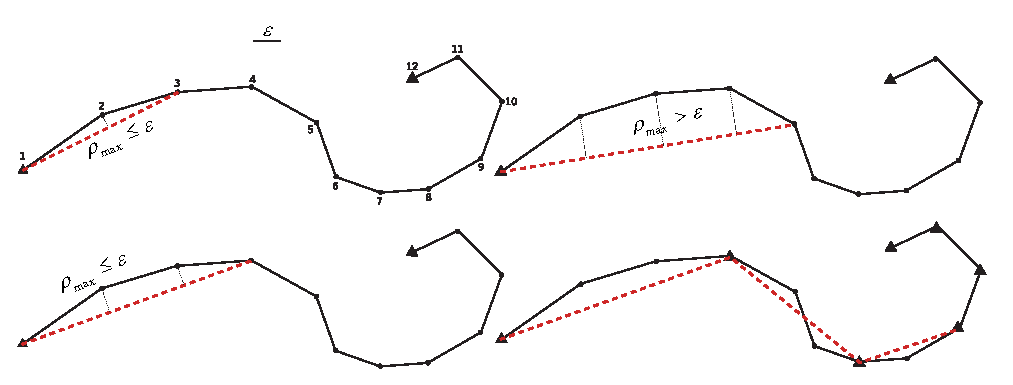
\includegraphics[width=1.0\linewidth]{img/iterative.eps}}
	\end{figure}
\end{frame}


\begin{frame}{Robust Variant}
	The robust modification of the non-recursive Douglas-Peucker technique 
	involves the detection of the possible intersections between:
	\begin{itemize}
		\item The new segments of the output line and the non-processed
			  segments of the original line.
		\item The new segments of the output line and the previous 
			  segments of the same output line.
	\end{itemize}		
\end{frame}	

\begin{frame}{Segment Intersection}
	\begin{figure}[h]
			\center{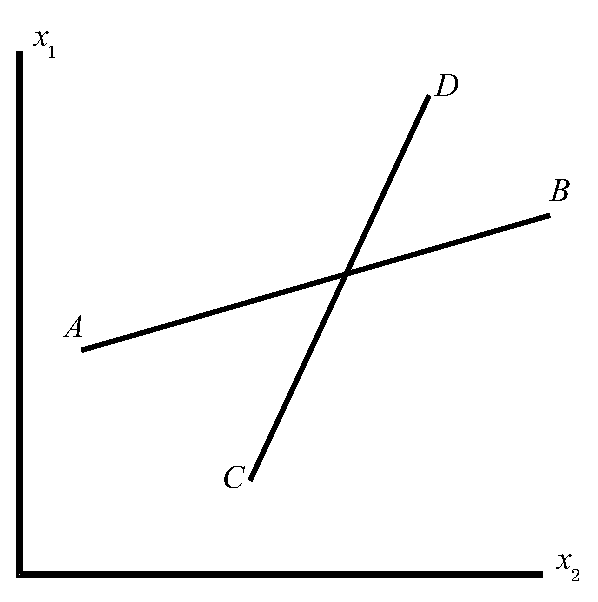
\includegraphics[width=0.4\linewidth]{img/intersection.eps}}
	\end{figure}
	\begin{align*}
					&	\overrightarrow{AB}\times\overrightarrow{AC} \cdot \overrightarrow{AB}\times\overrightarrow{AD} \leq 0 \\
	  \text{and } 	&	\overrightarrow{CD}\times\overrightarrow{CA} \cdot \overrightarrow{CD}\times\overrightarrow{CB} \leq 0 \\
	  \text{and } 	&	\overline{AB} \subset \overline{CD} \text{ or }  \overline{CD}  \subset \overline{AB} 	  	
	\end{align*}

\end{frame}


\begin{frame}{Example}
	\begin{figure}[h]
			\center{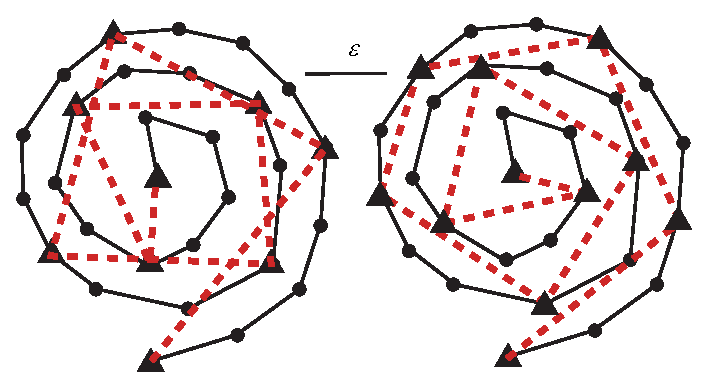
\includegraphics[width=1.0\linewidth]{img/robust.eps}}
	\end{figure}
\end{frame}



\end{document}
